\section{Introduction}\label{sec:introduction}

Distributed defense platforms increasingly split security execution across many servers while retaining centralized policy control. This arrangement improves local response speed, but it also exposes a decision bottleneck: once an observed request becomes ambiguous, a single classifier or a single large language model must determine whether to allow, monitor, or block it. Prior intrusion detection systems and modern AI-assisted detectors both suffer from this bottleneck in different forms. Classical systems such as Snort and Bro provide deterministic responses with limited semantic flexibility~\cite{roesch1999snort,paxson1999bro}, while learning-based detectors improve coverage but still concentrate judgment into one predictive boundary~\cite{doriguzzi2020lucid,neupane2022xids,holdbrook2024survey}. In operational web defense, this often translates into an undesirable trade-off: conservative thresholds raise false positives, whereas aggressive suppression of false alarms can undercut recall.

This paper positions \system\ around a narrower question than the broader platform literature: \emph{can role-specialized agent debate improve the triage of ambiguous web threats without losing auditability or distributed deployability?} The answer matters because security operators do not merely need labels. They also need a justification trail, a clear handling recommendation, and a record that can be reviewed after an escalation or a false alarm.

The repository already contains the ingredients for such a study. The backend exposes an authenticated agent gateway, HMAC-signed command dispatch, audit retention, configurable local/cloud/hybrid routing, and a multi-agent orchestration stack. More importantly, the current workspace contains a traceable public evaluation on an OWASP-derived benchmark slice and an explicit validated-capability snapshot. These artifacts support a paper that is more conservative, but also more defensible, than a platform-wide whitepaper.

Figure~\ref{fig:overview} summarizes the target argument of the paper. Rather than claiming that every subsystem of \system\ is independently novel, the draft centers one primary mechanism: debate-triggered security judgment over ambiguous web requests. The rest of the platform is presented only insofar as it supports that mechanism in a distributed setting.

\begin{figure}[t]
  \centering
  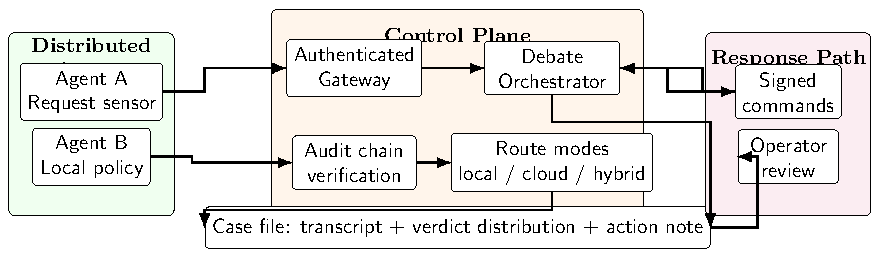
\includegraphics[width=\linewidth]{fig-system-overview.pdf}
  \caption{Overview of the paper's system-and-method scope.}
  \label{fig:overview}
\end{figure}

The paper makes three contributions.
\begin{enumerate}
  \item It defines a \textbf{role-specialized debate mechanism} for web threat triage in which Socrates performs adversarial challenge, Plato evaluates defensive handling, and Aristotle aggregates and arbitrates the final decision.
  \item It introduces an \textbf{auditable triage pipeline} that converts role outputs into a debate transcript, a final verdict distribution, and a case file suitable for post-incident review.
  \item It demonstrates these ideas in \textbf{the \system\ implementation} using repository-traceable public evidence: a 32-sample balanced OWASP-derived corpus and a validated smoke benchmark snapshot for system overhead.
\end{enumerate}

The remainder of the paper is organized as follows. Section~\ref{sec:related} reviews the three literature lines that matter for this narrowed thesis: web attack detection, AI-assisted security analysis, and multi-agent debate. Section~\ref{sec:method} formalizes the debate-driven triage method. Section~\ref{sec:system} maps that method onto the relevant \system\ implementation surfaces. Section~\ref{sec:evaluation} reports the public evidence layer and defines the protocol for a second, private labeled-alert layer. Section~\ref{sec:discussion} discusses limitations and concludes.
